\thispagestyle{quantoannone}
\pagestyle{quantoan}
\everymath{\color{quantoan}}
\graphicspath{{../quantoan/pic2/}}
\blfootnote{$^*$\color{quantoan}Nguồn https://plus.maths.org/content/does-infinity-exist?.}
\begingroup
\AddToShipoutPicture*{\put(0,616){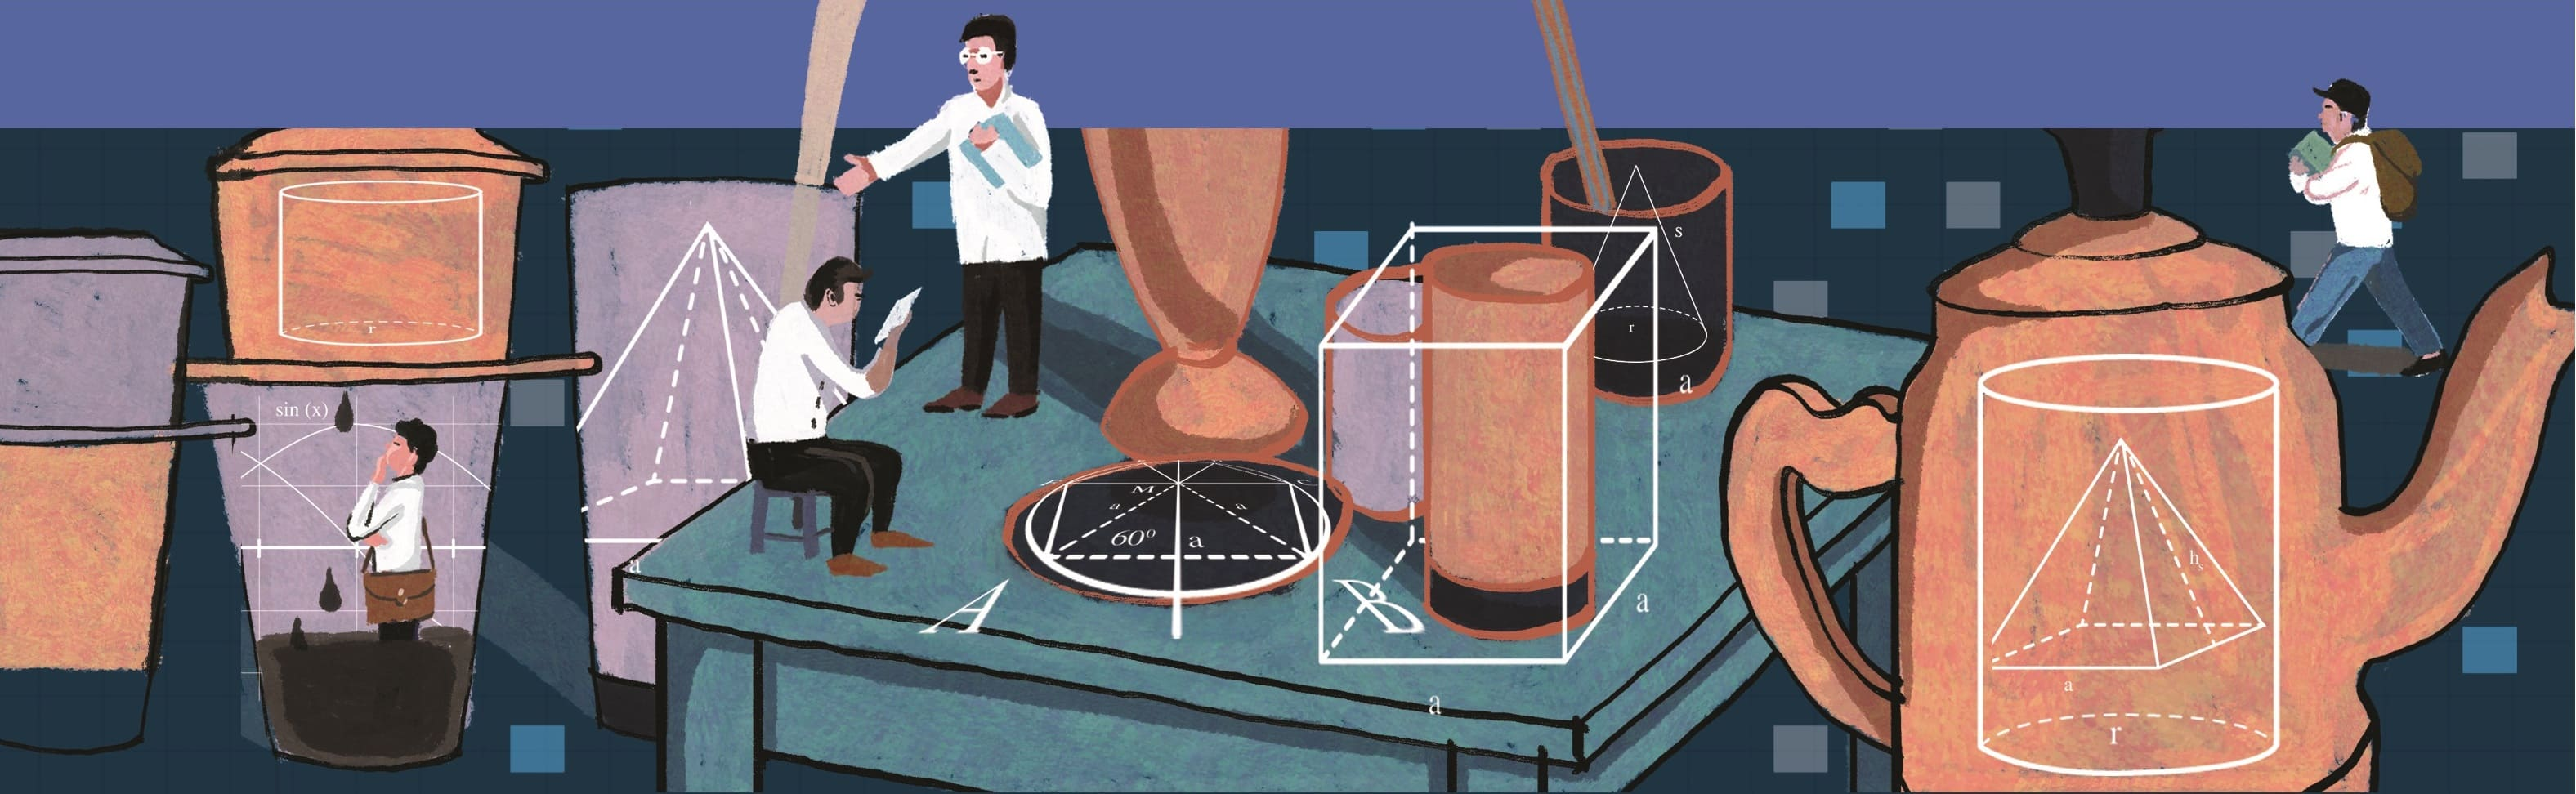
\includegraphics[width=19.3cm]{../bannerquantoan}}}
\AddToShipoutPicture*{\put(66,535){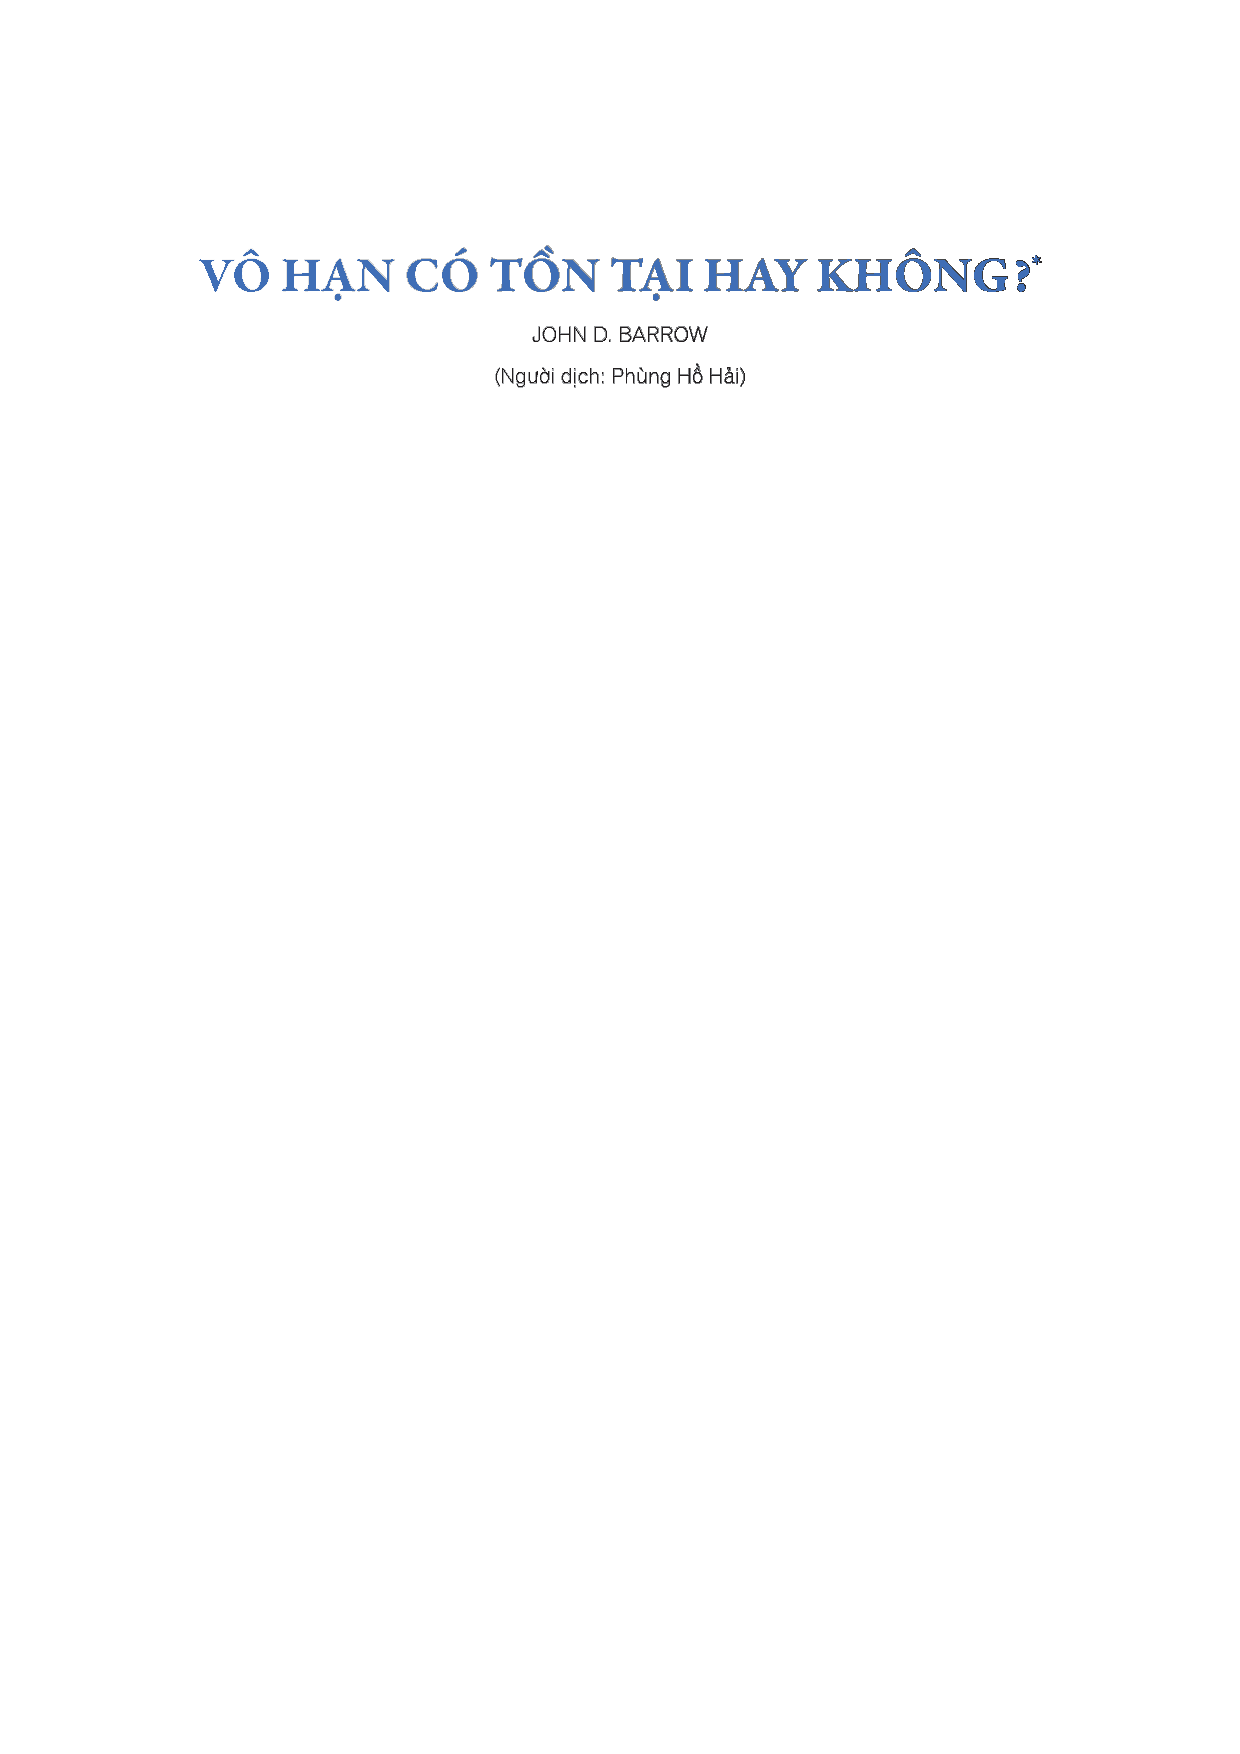
\includegraphics[scale=1]{../tieude1.pdf}}}
\centering
\endgroup

\vspace*{170pt}

\begin{multicols}{2}	
	Đây là một câu hỏi xưa đến bất ngờ. Aristotle là người đầu tiên làm rõ khái
	niệm này. Ông phân biệt hai dạng vô hạn. Một dạng được ông gọi là \textit{vô
	hạn tiềm năng}: đây là dạng vô hạn đặc trưng cho một Vũ trụ vô tận hoặc một
	danh sách vô tận, ví dụ như các số tự nhiên $1,2,3,4,5, \ldots$, tiếp diễn mãi
	mãi. Đây là những danh sách hoặc những mở rộng không có kết thúc hay biên
	giới: bạn không bao giờ có thể đạt đến tận cùng của tất cả các con số bằng
	cách liệt kê chúng, hoặc tận cùng của một vũ trụ vô tận bằng cách du hành trong
	một con tàu vũ trụ. Aristotle khá hài lòng về những vô hạn tiềm năng này, ông
	thừa nhận rằng chúng tồn tại và chúng không tạo ra bất kỳ mâu thuẫn lớn nào
	trong cách nghĩ của ông về Vũ trụ.
	\vskip 0.01cm
	Aristotle phân biệt dạng vô hạn tiềm năng với dạng mà ông gọi là \textit{vô
	hạn thực sự}. Đây sẽ là một cái gì đó bạn có thể đo lường, một cái gì đó cục
	bộ, chẳng hạn như mật độ của một chất rắn, hoặc độ sáng của một nguồn sáng, hoặc
	nhiệt độ của một vật thể, chúng là vô hạn tại một địa điểm hoặc thời gian cụ
	thể. Bạn sẽ có thể bắt gặp sự vô hạn này một cách cục bộ trong Vũ trụ. Aristotle cấm
	các vô hạn thực sự: ông nói rằng chúng không thể tồn tại. Điều này gắn liền
	với niềm tin khác của ông, rằng không thể có một chân không hoàn hảo trong tự
	nhiên. Nếu nó [chân không hoàn hảo] tồn tại, ông tin rằng bạn sẽ có thể đẩy và
	tăng tốc một vật thể đến tốc độ vô hạn vì nó sẽ không gặp phải lực cản nào.
	\vskip 0.1cm
	Trong vài nghìn năm, triết học của Aristotle đã củng cố cho các giáo điều và
	niềm tin của phương Tây và Cơ đốc giáo về bản chất của Vũ trụ. Mọi người tiếp
	tục tin rằng vô hạn thực sự không thể tồn tại, cụ thể hơn, vô hạn thực sự duy
	nhất được cho là tồn tại là thần thánh.
	\vskip 0.1cm
	\textbf{\color{quantoan}Vô hạn toán học}
	\vskip 0.1cm 
	Nhưng trong thế giới toán học, mọi thứ đã thay đổi vào cuối thế kỷ $19$ khi nhà
	toán học Georg Cantor phát triển một cách tinh tế hơn để xác định các dạng vô
	hạn trong toán học. Cantor nhận ra rằng có một kiểu vô hạn nhỏ nhất: danh sách
	vô tận của các số tự nhiên $1,2,3,4,5, \ldots$ Ông gọi đây là sự \textit{vô
		hạn đếm được}. Bất kỳ vô hạn nào khác có thể đếm được bằng cách đặt các
	thành viên của nó trong một tương ứng $1$--$1$ với các số tự nhiên cũng được gọi là
	vô hạn đếm được.
	\begin{center}
		$1 \longrightarrow 2$\\
		$2 \longrightarrow 4$\\
		$3 \longrightarrow 6$\\
		$4 \longrightarrow 8$\\
		\vskip 0.05cm
		\textit{\small\color{quantoan}Các số chẵn tương ứng một--một với các số~tự~nhiên.}
	\end{center}
	Ý tưởng này có một số hệ quả thú vị. Ví dụ, danh sách tất cả các số chẵn cũng
	là một vô hạn đếm được. Một cách trực giác, bạn có thể nghĩ rằng số số chẵn
	chỉ bằng một nửa số số tự nhiên bởi vì điều đó sẽ đúng với một danh sách hữu hạn.
	Nhưng khi danh sách trở thành vô tận điều đó không còn đúng nữa. Bạn có thể vẽ
	một đường nối từ $1$ đến $2$, từ $2$ đến $4$, và từ $3$ đến $6$, v.v. mãi
	mãi trong hai danh sách. Mọi số chẵn sẽ được nối với một và chỉ một số trong
	danh sách các số tự nhiên, vì vậy có bao nhiêu số trong danh sách này thì có
	bấy nhiêu 
	số trong danh sách kia. Điều này được nhận thấy đầu tiên bởi Galileo
	(mặc dù ông đếm các số chính phương $1, 4, 9, 16, \ldots$, chứ không phải các số
	chẵn), người thấy nó kỳ lạ đến mức khiến ông không thể nghĩ đến những tập
	hợp vô hạn nữa.  Ông nghĩ rằng có điều nghịch lý nguy hiểm nào đó về
	chúng. Tuy nhiên, đối với Cantor, việc có thể tạo ra một tương ứng một--một
	giữa một tập hợp các số và một tập hợp con của chúng là đặc tính xác định của
	một tập hợp vô hạn.
	\vskip 0.05cm 
	Tương tự, danh sách tất cả các số hữu tỷ, tức là tất cả các phân số, là một
	dạng vô hạn đếm được. Cách để đếm chúng một cách có hệ thống là cộng tử số và
	mẫu số, sau đó viết ra tất cả các phân số mà tổng này là $2$ (chỉ có một,
	$1/1$), sau đó viết tất cả các phân số mà tổng này là $3$ ($1/2$ và $2/1$),
	v.v. Mỗi lần bạn chỉ đếm một số hữu hạn phân số (số phân số $p / q$ mà
	$p + q = n$ là $n-1$). Đây là một quy tắc không thể sai để đếm tất cả các số
	hữu tỷ: bạn sẽ không bỏ sót bất kỳ số nào. Điều này cho thấy rằng các số hữu
	tỷ cũng có thể đếm được, mặc dù theo cảm nhận trực quan, dường như có nhiều
	số hữu tỷ hơn số tự nhiên rất nhiều.
	\vskip 0.05cm
	Cantor sau đó tiếp tục chỉ ra rằng còn có những dạng vô hạn khác mà theo một
	nghĩa nào đó lớn hơn vô hạn bởi vì chúng không thể được đếm theo cách này. Một
	dạng vô hạn như vậy là \emph{tập các số thực}. Tập này không thể đếm được; không có quy
	tắc để liệt kê chúng một cách có hệ thống. Vô hạn không đếm được này còn
	được gọi là \textit{liên tục} (\emph{continuum}).
	\vskip 0.05cm
	Nhưng câu chuyện chưa dừng lại ở việc tìm ra tập hợp các số thực lớn hơn vô
	hạn này. 
	Cantor đã chỉ ra rằng bạn vẫn có thể tìm thấy những dạng
	vô hạn lớn hơn nữa, và cứ tiếp tục mãi như vậy: không có tập vô hạn lớn nhất.
	Nếu ai đó cho bạn một tập hợp vô hạn $A$, bạn có thể tạo ra
	một tập hợp lớn hơn mà không thể tương ứng $1$--$1$ với $A$, đơn giản
	bằng cách lấy tập hợp tất cả các tập con của $A$. Tháp vô hạn không bao giờ
	kết thúc này hướng tới thứ gọi là \emph{vô hạn tuyệt đối} -- một đỉnh không thể chạm
	tới của tháp vô hạn. (Bạn có thể tìm hiểu thêm về công trình của Cantor trong
	bài \textit{Một thoáng thiên đường của Cantor\footnote{\color{quantoan}A glimpse of Cantor's
			paradise, https://plus.maths.org/content/glimpse-cantors-paradise}}, trên
	Plus.)
	\vskip 0.05cm
	Về mặt toán học, Cantor coi các dạng vô hạn không chỉ là tiềm năng mà còn là
	thực sự. Bạn có thể cộng chúng lại với nhau -- một vô hạn đếm được cộng
	với một vô hạn đếm được khác là một vô hạn đếm được -- v.v. Đã có
	một cuộc tranh cãi lớn trong toán học về việc liệu điều này có nên được phép
	hay không. Một số nhà toán học nghĩ rằng bằng cách cho phép các
	\emph{đại lượng siêu hạn} (\emph{transfinite quantities}) của Cantor, 
	như cách chúng được gọi vào thời đó, vào toán học, bạn đang
	đưa vào đâu đó một mâu thuẫn tinh vi. Và nếu bạn đưa các mâu thuẫn vào một hệ
	thống logic, thì cuối cùng bạn sẽ có thể chứng minh rằng mọi điều là
	đúng, vì vậy nó sẽ dẫn đến sự sụp đổ của toàn bộ hệ thống toán học.
	\vskip 0.05cm
	Lo lắng này đã dẫn đến khái niệm \emph{toán học hữu hạn} (\emph{finitist}) hoặc 
	\emph{toán học kiến tạo} (\emph{constructivist}), 
	chỉ cho phép các đối tượng toán học có thể xây dựng bằng một
	chuỗi hữu hạn các lập luận logic. Toán học của bạn sau đó trở nên giống như
	những gì máy tính có thể làm. Bạn đặt ra một số tiên đề và chỉ những
	thứ có thể được suy ra từ chúng bằng một chuỗi hữu hạn các bước logic mới được
	coi là đúng. Điều này có nghĩa là bạn không được phép sử dụng chứng minh phản
	chứng (còn gọi là luật bài trung) như một tiên đề: giả thiết rằng một cái gì đó
	không tồn tại, từ đó suy ra mâu thuẫn để kết luận rằng nó phải tồn tại. Những
	nhà toán học thế kỷ XIX ủng hộ quan điểm kiến tạo này là nhà toán học người Hà
	Lan LEJ Brouwer và Leopold Kroneker, và trong thế kỷ XX, Hermann Weyl đã 
	có một thời gian quan tâm đến nó. Vẫn có một số nhà toán học muốn định nghĩa
	toán học theo cách này vì lý do triết học, và một số người khác chỉ quan tâm
	đến những gì bạn có thể chứng minh nếu bạn định nghĩa nó theo cách hạn chế
	này. (Để tìm hiểu thêm về điều này, hãy đọc bài \textit{Toán học kiến
	thiết}\footnote{\color{quantoan}Constructive maths,
		https://plus.maths.org/content/constructive-mathematics}  trên Plus.)
	\vskip 0.05cm
	Nhưng nhìn chung các ý tưởng của Cantor đã được chấp nhận và ngày nay chúng
	hình thành nhánh con của riêng mình trong toán học thuần túy. Điều này đã
	khiến một số nhà triết học, và thậm chí một số nhà thần học, suy nghĩ lại về
	thái độ cổ xưa của họ đối với sự vô hạn. Bởi vì có khá nhiều dạng vô hạn khác
	nhau, rõ ràng là bạn không cần phải coi sự xuất hiện của vô hạn toán học là
	một thách thức đối với thần thánh như các nhà thần học thời Trung cổ đã tin
	tưởng. Những ý tưởng của Cantor lúc đầu thực sự được các nhà thần học đương
	thời tiếp thu nhiệt tình hơn là các nhà toán học.
	\vskip 0.05cm
	Các nhà khoa học cũng bắt đầu phân biệt giữa các vô hạn toán học và vật lý.
	Trong toán học, nếu bạn nói một cái gì đó ``tồn tại'', ý bạn là sự tồn tại đó
	không tạo ra mâu thuẫn logic với một bộ quy tắc cụ thể. Nhưng nó không có
	nghĩa là bạn có cái đó trên bàn của mình hoặc đang ``chạy quanh đâu đó''. Kỳ lân
	không phải là một thứ bất khả thi về mặt logic nhưng điều đó không có nghĩa
	là một con kỳ lân tồn tại về mặt sinh học. Khi các nhà toán học chứng minh
	rằng các hình học phi Euclid có thể tồn tại, họ đã chỉ ra rằng có một hệ tiên
	đề cho phép chúng mà không tự mâu thuẫn. (Bạn có thể tìm hiểu thêm về các hình
	học phi Euclide trong bài viết \textit{Hình học kỳ lạ}\footnote{\color{quantoan}Strange geometries,
		https://plus.maths.org/content/mathematical-mysteries-strange-geometries}.)
	\vskip 0.05cm
	\textbf{\color{quantoan}Vô hạn vật lý}
	\vskip 0.05cm 
	Như vậy, vô hạn trong vật lý hiện đại tách biệt với vô hạn trong toán học. Một
	lĩnh vực trong vật lý nơi các dạng vô hạn đôi khi được dự đoán sẽ phát sinh là
	khí động học hoặc cơ học chất lưu. Ví dụ, bạn có thể có một sóng trở nên
	rất, rất dốc và phi tuyến tính và sau đó tạo thành một sóng xung kích. Trong các
	phương trình mô tả sự hình thành sóng xung kích, một số đại lượng có thể trở
	nên vô hạn. Nhưng khi điều này xảy ra, bạn thường cho rằng đó chỉ là một sự
	thất bại của mô hình của mình. Bạn có thể đã bỏ qua việc tính đến ma sát hoặc
	độ nhớt và một khi bạn đưa điều đó vào phương trình của mình thì gradient vận
	tốc trở nên hữu hạn -- nó có thể vẫn rất dốc, nhưng độ nhớt trong thực tế thì
	sẽ làm mịn đi tính vô hạn. Trong hầu hết các lĩnh vực khoa học, nếu bạn nhìn
	thấy vô hạn, bạn cho rằng đó là do mô hình của bạn không chính xác hoặc không
	đầy đủ.
	\begin{figure}[H]
		\centering
		\vspace*{-5pt}
		\captionsetup{labelformat= empty, justification=centering}
		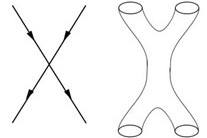
\includegraphics[width=0.75\linewidth]{1}
		\caption{\small\textit{\color{quantoan}Hai hạt gặp nhau tạo thành một góc nhọn (trái) nhưng
				hai vòng lại gần với nhau giống như hai chiếc quần được khâu vào nhau. (Sơ đồ
				ống quần có thời gian đi xuống và không gian nằm ngang.)}}
		\vspace*{-10pt}
	\end{figure}
	Trong vật lý hạt, có một vấn đề tồn tại lâu đời hơn và phức tạp hơn. Điện
	động lực học lượng tử là lý thuyết tốt nhất trong toàn bộ khoa học, các dự
	đoán của nó chính xác hơn bất cứ điều gì khác mà chúng ta biết về Vũ trụ. Tuy
	nhiên, việc trích xuất những dự đoán đó lại đưa ra một vấn đề khó xử: khi bạn
	tính toán để xem những gì bạn có thể quan sát thấy trong một thí nghiệm,
	dường như bạn luôn nhận được câu trả lời vô hạn với một chút hữu hạn được thêm
	vào. Sau đó, nếu bạn trừ đi phần vô hạn, thì phần hữu hạn còn lại là dự
	đoán mà bạn mong đợi sẽ thấy trong phòng thí nghiệm. Và dự đoán này luôn
	khớp với thí nghiệm một cách chính xác đến kinh ngạc. 
	Quá trình loại bỏ các vô hạn này được gọi là \emph{tái chuẩn hóa}. 
	Nhiều nhà vật lý nổi tiếng rất không hài lòng với nó.
	Họ nghĩ rằng đó có thể chỉ là dấu hiệu rằng lý thuyết có thể
	được tiếp tục cải thiện.
	\vskip 0.05cm
	Đây là lý do tại sao lý thuyết dây tạo ra sự phấn khích lớn trong những năm
	$1980$ và tại sao nó đột nhiên được rất nhiều các nhà vật lý nghiên cứu.
	Đây là lần đầu tiên các nhà vật lý hạt tìm ra một lý thuyết hữu hạn, một
	lý thuyết không xuất hiện những vô hạn. Đề xuất của lý thuyết này là thay thế
	quan niệm truyền thống rằng các thực thể cơ bản nhất trong lý thuyết (ví dụ
	như photon hoặc electron) phải là các đối tượng dạng điểm di chuyển trong
	không gian và thời gian và do đó vạch ra các đường trong không--thời gian.
	Thay vào đó, lý thuyết dây coi các thực thể cơ bản nhất là các đường, hoặc các
	vòng nhỏ, vạch ra các ống khi chúng di chuyển. Khi bạn có hai hạt dạng điểm
	di chuyển trong không gian và tương tác với nhau, nó giống như hai đường thẳng
	va vào nhau và tạo thành một góc nhọn tại nơi chúng gặp nhau. 
	Góc nhọn trong hình vẽ chính là nguồn gốc của sự vô hạn.
	Nhưng nếu bạn có
	hai vòng dây gần nhau, nó giống như hai ống quần của một chiếc quần. Sau đó,
	hai vòng nữa di chuyển ra từ tương tác -- điều đó giống như việc may một
	chiếc quần khác vào chiếc đầu tiên. Những gì bạn nhận được là một quá trình
	chuyển đổi suôn sẻ. Đây là lý do tại sao lý thuyết dây rất hấp dẫn, nó là lý
	thuyết hữu hạn đầu tiên của vật lý hạt.
	\vskip 0.05cm
	\textbf{\color{quantoan}Vô hạn vũ trụ} 
	\vskip 0.05cm
	Một dạng vô hạn khác nảy sinh trong lý thuyết hấp dẫn và vũ trụ học
	(cosmology). Thuyết tương đối rộng của Einstein cho rằng một Vũ trụ đang dãn
	nở (như chúng ta quan sát thấy trong Vũ trụ của chúng ta) bắt đầu vào một thời điểm
	trong quá khứ hữu hạn khi mật độ của nó là vô hạn -- đây là cái mà chúng ta
	gọi là Vụ nổ lớn. Lý thuyết của Einstein cũng dự đoán rằng nếu bạn rơi vào một
	lỗ đen, và có nhiều lỗ đen trong Ngân Hà của chúng ta và lân cận, bạn sẽ gặp
	phải mật độ vô hạn ở trung tâm. Các dạng vô hạn này, nếu chúng tồn tại, sẽ là
	các vô hạn thực~sự.
	\begin{figure}[H]
		\centering
		\vspace*{-5pt}
		\captionsetup{labelformat= empty, justification=centering}
		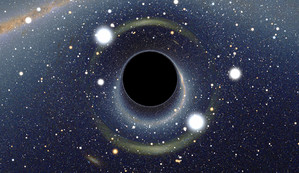
\includegraphics[width=1\linewidth]{2}
		\caption{\small\textit{\color{quantoan}Hình ảnh mô phỏng của một lỗ đen. Ảnh: Alain Riazuelo.}}
		\vspace*{-10pt}
	\end{figure}
	Người ta có thái độ khác nhau đối với dạng vô hạn này. Các nhà vũ trụ học xuất
	thân từ vật lý hạt và quan tâm đến giải thích của lý thuyết dây về sự khởi đầu của Vũ
	trụ sẽ có xu hướng cho rằng những vô hạn này không có thật, rằng chúng chỉ là
	một giả tượng của đặc tính chưa hoàn thiện của lý thuyết hiện có. Có những người
	khác, ví dụ Roger Penrose, cho rằng xuất phát vô hạn ở thuở ban đầu của Vũ trụ
	đóng một vai trò rất quan trọng trong cấu trúc của vật lý. Nhưng ngay cả khi
	những vô hạn này là một giả tượng, thì mật độ vẫn trở nên cao đến kinh ngạc: lớn
	gấp $10^{96}$ lần mật độ của nước. Thực tế, nó cao
	đến mức chúng ta cần một mô tả về tác động của lý thuyết lượng tử đối với đặc
	tính của không gian, thời gian và lực hấp dẫn để hiểu được điều gì đang diễn
	ra ở đó.
	\vskip 0.05cm
	Một điều gì đó rất kỳ quặc có thể xảy ra nếu chúng ta giả định rằng Vũ trụ của
	chúng ta cuối cùng sẽ ngừng mở rộng và co lại về một vô hạn khác, một
	\textit{vụ co lớn}. Vụ co lớn đó có thể xảy ra không đồng thời bởi vì một số
	phần của Vũ trụ, nơi có các thiên hà, v.v., dày đặc hơn những phần khác. Những
	nơi có mật độ dày đặc hơn sẽ trở thành vô hạn trước những vùng
	có mật độ thấp. Nếu chúng ta đang ở trong một khoảng Vũ trụ mà tương
	lai vô hạn xảy ra muộn hơn, hoặc thậm chí không xảy ra, thì chúng ta có thể
	nhìn lại và thấy sự kết thúc của Vũ trụ ở những nơi khác -- chúng ta sẽ thấy
	một thứ gì đó vô hạn. Bạn có thể thấy bằng chứng về không gian và thời gian
	sắp kết thúc ở nơi khác.
	\vskip 0.05cm
	Nhưng thật khó để dự đoán chính xác những gì bạn sẽ thấy nếu một vô hạn thực
	sự xuất hiện ở đâu đó. Cách Vũ trụ của chúng ta được thiết lập ở hiện tại
	có một cơ chế bảo vệ thú vị. Một cách giải thích đơn giản về sự vật cho
	thấy rằng có một mật độ vô hạn xuất hiện ở trung tâm của mỗi lỗ đen, giống như
	vô hạn ở kết thúc của Vũ trụ. Nhưng một lỗ đen tạo ra một chân trời sự kiện
	xung quanh hiện tượng này: ngay cả ánh sáng cũng không thể thoát ra khỏi vùng
	lân cận của nó. Vì vậy, chúng ta bị cách ly, chúng ta không thể nhìn thấy
	những gì đang xảy ra ở những nơi mà mật độ dường như sẽ trở nên vô hạn. Và cả
	vô hạn đó cũng không thể ảnh hưởng đến chúng ta. Những chân trời sự kiện này bảo vệ chúng ta khỏi hệ quả của những nơi mà mật độ có thể là vô hạn và chúng ngăn
	chúng ta nhìn thấy những gì đang diễn ra ở đó, tất nhiên trừ khi chúng ta đang
	ở bên trong một lỗ đen.
	\vskip 0.05cm
	Một câu hỏi khác là liệu Vũ trụ của chúng ta là hữu hạn hay vô hạn về không
	gian. Tôi nghĩ rằng chúng ta không bao giờ có thể biết được. Nó có thể là hữu
	hạn nhưng có kích thước lớn tùy ý. Nhưng đối với nhiều người, ý tưởng về một
	Vũ trụ hữu hạn ngay lập tức đặt ra câu hỏi về những gì bên ngoài nó. Không có
	bên ngoài -- Vũ trụ là tất cả mọi thứ ở đó. Để hiểu điều này, chúng ta hãy
	nghĩ đến các vũ trụ hai chiều vì chúng dễ hình dung hơn. Nếu chúng ta cầm một
	tờ giấy A$4$ lên, chúng ta thấy nó có cạnh, vậy làm sao vũ trụ hữu hạn lại
	không có cạnh? Nhưng vấn đề là mảnh giấy phẳng. Nếu chúng ta nghĩ về một bề
	mặt hai chiều khép kín và cong, giống như một mặt cầu, thì diện
	tích của mặt cầu là hữu hạn: bạn chỉ cần một lượng sơn hữu hạn để sơn nó.
	Nhưng nếu bạn đi bộ xung quanh nó, không như với mảnh giấy phẳng, bạn sẽ
	không bao giờ gặp phải một cạnh. Vì vậy không gian cong có thể là hữu hạn
	nhưng không có ranh giới hoặc cạnh.
	\begin{figure}[H]
		\centering
		\vspace*{-5pt}
		\captionsetup{labelformat= empty, justification=centering}
		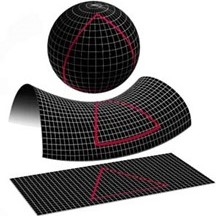
\includegraphics[width=0.77\linewidth]{3}
		\caption{\small\textit{\color{quantoan}Mặt cầu có độ cong dương, hình yên ngựa có độ cong âm
				và mặt phẳng có độ cong bằng không. Các tam giác được tạo thành bằng cách vẽ
				các đường ngắn nhất giữa các cặp điểm. Khi tổng các góc vượt quá (nhỏ hơn)
				$180$ độ thì bề mặt có độ cong dương (âm). Khi nó bằng $180$ độ, bề mặt phẳng,
				không có độ cong. Hình ảnh do NASA cung cấp.}}
		\vspace*{-10pt}
	\end{figure}
	Để hiểu về một Vũ trụ hai chiều đang dãn nở, trước tiên chúng ta hãy nghĩ đến
	trường hợp vô hạn, trong đó Vũ trụ trông giống nhau ở bất kỳ đâu bạn tới. Khi
	đó, bất cứ nơi nào bạn đứng và nhìn xung quanh mình, có vẻ như Vũ trụ đang mở
	rộng ra xa với bạn ở trung tâm bởi vì mọi nơi đều giống như trung tâm. Đối với một
	vũ trụ hình cầu hữu hạn, hãy tưởng tượng hình cầu như một quả bóng bay với các
	thiên hà được đánh dấu trên bề mặt. Khi bạn bắt đầu thổi phồng nó, các thiên
	hà bắt đầu rời xa nhau. Dù đứng ở bất cứ nơi nào trên bề mặt của quả cầu, bạn
	cũng sẽ thấy tất cả các thiên hà khác đang dãn ra khỏi bạn khi cao su nở ra. Tâm
	của sự mở rộng không nằm trên bề mặt, nó nằm trong một không gian khác, trong
	trường hợp này là chiều thứ ba. Vì vậy, Vũ trụ ba chiều của chúng ta, nếu nó
	là hữu hạn và độ cong dương, sẽ hoạt động như thể đó là bề mặt ba chiều của
	một quả bóng bốn chiều tưởng tượng.
	\vskip 0.05cm
	Einstein nói với chúng ta rằng hình dạng của không gian được xác định bởi mật
	độ vật chất trong đó. Giống như tấm bạt lò xo cao su: nếu bạn đặt vật liệu lên
	tấm bạt lò xo, nó sẽ biến dạng độ cong. Nếu có nhiều vật chất trong không
	gian, nó sẽ gây ra sự lõm xuống rất lớn và không gian co lại. Vì vậy, một
	Vũ trụ mật độ cao yêu cầu một dạng hình cầu và nó sẽ có thể tích hữu hạn.
	Nhưng nếu bạn có tương đối ít vật liệu để làm biến dạng không gian,
	bạn sẽ có một không gian \emph{có độ cong âm}, có hình dạng như yên ngựa hoặc lát khoai tây
	chiên giòn. Một không gian cong âm như vậy có thể tiếp tục bị kéo dãn và mở
	rộng mãi mãi. Một Vũ trụ mật độ thấp, nếu nó có dạng hình học đơn giản, sẽ có
	kích thước và thể tích vô hạn. Nhưng nếu nó có một cấu trúc liên kết kỳ lạ
	hơn, như một hình xuyến, thì nó cũng có thể có một thể tích hữu hạn. Một trong
	những bí ẩn về các phương trình của Einstein là chúng cho bạn biết làm thế nào
	để tính toán hình dạng từ sự phân bố của vật chất, nhưng các phương
	trình của ông không nói gì về cấu trúc liên kết của Vũ trụ. Có thể một
	lý thuyết sâu hơn về lực hấp dẫn lượng tử sẽ có thể nói về điều đó.
	\vskip 0.05cm
	\textbf{\color{quantoan}Về tác giả}
	\vskip 0.05cm
	John D. Barrow là Giáo sư Khoa học Toán học tại Đại học Cambridge, tác giả của
	nhiều cuốn sách khoa học phổ biến và là giám đốc của Dự án Toán học Thiên niên
	kỷ, mà Plus là một phần trong đó.
	\vskip 0.05cm
	Barrow là tác giả của \textit{Cuốn sách vô hạn: Hướng dẫn ngắn gọn về sự vô
	biên, vượt thời gian và vô tận}, cho bạn biết thêm nhiều điều về vô hạn.
	\textit{Cuốn sách về các vũ trụ} của ông cũng có liên quan đến phần cuối về vũ
	trụ học và lý thuyết dây của bài viết này.
\end{multicols}
\vspace*{-10pt}
\rule{1\linewidth}{0.1pt}
\begin{center}
	\textbf{\Large\color{quantoan}LỜI GIẢI, ĐÁP ÁN}
\end{center}
\begin{multicols}{2}
	\textbf{\color{quantoan}Bác nông dân tốt bụng}
	\begin{figure}[H]
			\vspace*{-5pt}
			\centering
			\captionsetup{labelformat= empty, justification=centering}
			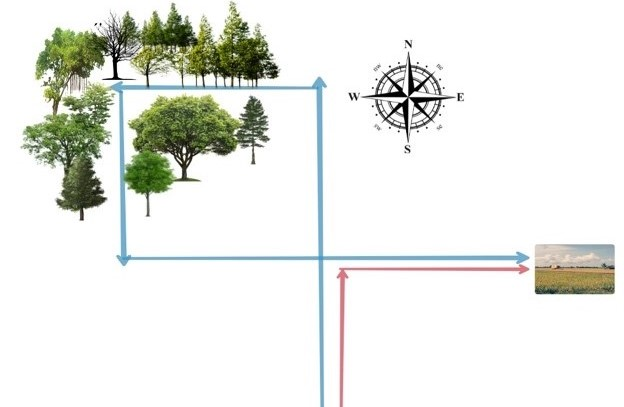
\includegraphics[width= 0.95\linewidth]{lgxp}
			\vspace*{-10pt}
		\end{figure}
	Do bác nông dân đi xuyên qua rừng với vận tốc bằng nửa so với vận tốc đi trên đường cái, nên trong hai ngày đêm (thứ hai và thứ ba) bác chỉ đi được quãng đường bằng quãng đường đi được trong cả ngày đêm thứ nhất, có nghĩa là một phần ba quãng đường. Vì thế $30$ km đi được trong ngày và đêm thứ tư cũng chính là $1/3$ quãng đường. Vậy bác nông dân đã đi hết $90$ km. Con đường đi của bác nông dân được biểu diễn bằng màu xanh như trên hình vẽ. 
	\vskip 0.05cm
	Xuân Phong đã lập luận như sau: nếu chỉ đi nửa đoạn đường lên phía bắc rồi quay ngay 	sang hướng đông, thì chỉ hết nửa ngày nữa là thám tử đã đến Vườn Ngô, sau khi đi nửa quãng đường về phía bắc và nửa quãng đường về phía đông, có nghĩa là thám tử chỉ cần đi có $30$ km (theo con đường màu đỏ). 
	\vskip 0.1cm
	\hfill (\textit{Xem tiếp trang} $33$.)
%	\textbf{\color{thachthuctoanhoc}Đố vui}
%	\vskip 0.05cm 
%	Có thể dễ dàng chỉ ra rằng với hai chiếc máy bay, Pi không thể thực hiện được kế hoạch của mình. Với ba chiếc máy bay thì Pi có thể thực hiện được, chẳng hạn với chiến lược sau đây.   
%	\vskip 0.05cm
%	Đầu tiên, ba máy bay, một chiếc của Pi và hai chiếc khác để hỗ trợ Pi, cùng xuất phát từ sân bay. Sau khi đi được $1/8$ vòng Trái Đất, một máy bay tiếp nhiên liệu cho cả máy bay của Pi và chiếc còn lại, mỗi chiếc $1/4$ bình (nếu coi mỗi chiếc máy bay có $1$ bình nhiên liệu) và giữ lại cho mình $1/4$ bình. Khi này, hai chiếc máy bay có đầy bình và một chiếc có $1/2$ bình (vừa đủ để có thể quay lại sân bay ban đầu). Sau đó, hai máy bay có đầy bình tiếp tục hành trình của mình còn chiếc còn $1/2$ bình quay trở lại sân bay ban đầu. 
%	\vskip 0.05cm
%	Sau khi tiếp tục đi được $1/8$ vòng Trái Đất, nghĩa là được $1/4$ vòng kể từ điểm xuất phát, chiếc còn lại chuyển $1/4$ bình nhiên liệu cho Pi. Khi này Pi có đầy bình và chiếc còn lại có $1/4$ bình, vừa đủ để quay trở lại. Bây giờ, Pi tiếp tục hành trình của mình còn chiếc máy bay kia quay trở lại sân bay ban đầu. Với đầy bình, Pi có thể đi được $3/4$ vòng Trái Đất kể từ điểm xuất phát. 
%	\vskip 0.05cm
%	Máy bay đầu tiên, với đầy bình bay theo hướng ngược lại (so với hướng ban đầu) để gặp máy bay của Pi ở vị trí $3/4$ vòng Trái Đất, khi đó máy bay đầu tiên còn ½ bình sẽ tiếp cho máy bay của Pi $1/4$ bình, sao cho cả hai máy bay có $1/4$ bình, đủ để đi đến vị trí $7/8$ vòng Trái Đất. Khi hai chiếc máy bay này gặp nhau, chiếc còn lại bắt đầu xuất phát từ sân bay ban đầu với đầy bình và bay theo hướng ngược lại để gặp máy bay của Pi và chiếc thứ hai ở vị trí $7/8$ vòng Trái Đất và tiếp cho mỗi chiếc $1/4$ bình. Khi này, mỗi chiếc có đúng $1/4$ bình, vừa đủ để bay về sân bay ban đầu.   
%	\vskip 0.05cm
%	\textbf{Góc cờ}
%	\vskip 0.05cm
%	\textbf{\color{gocco}Bài $\pmb{1}$.
%		$\pmb{1}$.Vd$\pmb{4}$ Vb$\pmb{4}$ $\pmb{2}$.Xg$\pmb{2}$ Mh$\pmb{3}$} [$2$...Md$1$ $3$.Xd$2$]
%	\vskip 0.05cm
%	\textbf{\color{gocco}$\pmb{3}$.Ke$\pmb{3}$} Mã đen bị bắt.
%	\vskip 0.05cm
%	\textbf{\color{gocco}Bài $\pmb{2}$. 
%		$\pmb{1}$.Vc$\pmb{4}$ Vc$\pmb{6}$} [$1$...Mh$3$ $2$.Xg$4$ Mf$2$ $3$.Xh$4$]
%	\vskip 0.05cm
%	\textbf{\color{gocco}$\pmb{2}$.Xh$\pmb{4}$ Vd$\pmb{6}$ $\pmb{3}$.Vd$\pmb{4}$ Ve$\pmb{6}$ $\pmb{4}$.Ve$\pmb{3}$ Md$\pmb{1+}$ $\pmb{5}$.Vd$\pmb{2}$ Mb$\pmb{2}$} [$5$...Mf$2$ $6$.Ve$2$]
%	\vskip 0.05cm
%	\textbf{\color{gocco}$\pmb{6}$.Xb$\pmb{4}$}
%	\vskip 0.05cm
%	\textbf{\color{gocco}Bài $\pmb{3}$.
%		$\pmb{1}$.Xd$\pmb{4}$!! Mb$\pmb{6}$} [$1$...Mb$2$ $2$.Ve$3$ Vf$5$ $3$.Vd$2$ Ve$5$ $4$.Xb$4$]
%	\vskip 0.05cm
%	\textbf{\color{gocco}$\pmb{2}$.Ve$\pmb{5}$ Mc$\pmb{8}$ $\pmb{3}$.Ve$\pmb{6}$ Ma$\pmb{7}$ $\pmb{4}$.Vd$\pmb{7}$ Mb$\pmb{5}$} [$4$...Vf$5$ $5$.Xa$4$ Mb$5$ $6$.Xa$5$; $4$...Vg$6$ $5$.Xd$5$]
%	\vskip 0.05cm
%	\textbf{\color{gocco}$\pmb{5}$.Xd$\pmb{5+}$}
%	\vskip 0.05cm
%	$\pmb{1-0}$
\end{multicols}